% Author: Dominik Harmim <xharmi00@stud.fit.vutbr.cz>

\documentclass[a4paper, 11pt]{article}

\usepackage[czech]{babel}
\usepackage[utf8]{inputenc}
\usepackage[left=2cm, top=3cm, text={17cm, 24cm}]{geometry}
\usepackage{times}
\usepackage{graphicx} % vkládání obrázků
\usepackage[unicode]{hyperref}
\hypersetup{
	colorlinks = true,
	hypertexnames = false,
	citecolor = red
}

\newcommand{\RNum}[1]{\uppercase\expandafter{\romannumeral #1\relax}} % makro na sázení římských čísel

\begin{document}

	%%%%%%%%%%%%%%%%%%%%%%%%%%%%%%%% Titulní stránka %%%%%%%%%%%%%%%%%%%%%%%%%%%%%%%%
	\begin{titlepage}
		\begin{center}
			
\includegraphics[width=0.77\linewidth]{inc/FIT_logo.pdf} \\

			\vspace{\stretch{0.382}}

			\Huge{Projektová dokumentace} \\
			\LARGE{\textbf{Implementace překladače imperativního jazyka IFJ17}} \\
			\Large{Tým 104, varianta \RNum{2}}
			\vspace{\stretch{0.618}}
		\end{center}

		\begin{minipage}{0.4 \textwidth}
			{\Large \today}
		\end{minipage}
		\hfill
		\begin{minipage}[r]{0.6 \textwidth}
			\Large
			\begin{tabular}{l l l}
				\textbf{Dominik Harmim} & \textbf{(xharmi00)} & \quad 25\,\% \\
				Vojtěch Hertl & (xhertl04) & \quad 25\,\% \\
				Timotej Halás & (xhalas10) & \quad 25\,\% \\
				Matej Karas & (xkaras34) & \quad 25\,\% \\
			\end{tabular}
		\end{minipage}
	\end{titlepage}


	%%%%%%%%%%%%%%%%%%%%%%%%%%%%%%%% Obsah %%%%%%%%%%%%%%%%%%%%%%%%%%%%%%%%
	\pagenumbering{roman}
	\setcounter{page}{1}
	\tableofcontents
	\newpage


	%%%%%%%%%%%%%%%%%%%%%%%%%%%%%%%% Úvod %%%%%%%%%%%%%%%%%%%%%%%%%%%%%%%%
	\pagenumbering{arabic}
	\setcounter{page}{1}

	\section{Úvod}

	Cílem projektu bylo vytvořit program v~jazyce C, který načte zdrojový kód zapsaný ve zdrojovém jazyce IFJ17,
	jenž je zjednodušenou podmnožinou jazyka FreeBASIC a~přeloží jej do cílového jazyka IFJcode17 (mezikód).


	%%%%%%%%%%%%%%%%%%%%%%%%%%%%%%%% Návrh a implementace %%%%%%%%%%%%%%%%%%%%%%%%%%%%%%%%
	\section{Návrh a~implementace}

	\subsection{Lexikální analýza}

	TODO


	\subsection{Syntaktická analýza}

	TODO


	\subsection{Sémantická analýza}

	TODO


	\subsection{Optimalizace}

	TODO


	\subsection{Generování cílového kódu}

	TODO


	\subsection{Překladový systém}

	Projekt je možné přeložit dvěma způsoby, buď nástrojem CMake nebo nástrojem GNU Make. Oba způsoby vytvoří
	spustitelný soubor \texttt{ifj17\_compiler}.

	\subsubsection{CMake}

	Při vývoji, ladění a~testování projketu někteří z~nás používaly CMake, protože překlad tímto nástrojem
	je integrován ve vývojovém prostředí CLion, které většina členů týmu používala a~protože nastavení pravidel
	pro překlad tímto nástrojem je jednoduché.

	V~souboru \texttt{CMakeLists.txt} jsou nastavena pravidla pro překlad. Je zde nastaven překladač \texttt{gcc}
	a~všechny potřebné parametry pro překlad. Dále je zde uvedeno, že se pro překlad mají používít všechny soubory s~příponou
	\texttt{.c} a~\texttt{.h} a~taky je zde uveden název spustitelného souboru.

	Soubory pro překlad je možné vygenerovat příkazem \texttt{cmake~.} a~překlad provést příkazem \texttt{cmake~--build~.}
	nebo pro toto využít nástroje vývojového prostředí.

	\subsubsection{GNU Make}

	Jedním z~požadavdků pro odevzdání projektu bylo přiložit k~odevzdanému projektu i~soubor \texttt{Makefile} a~přeložení
	projektu příkazem \texttt{make}. Z~tohoto důvodu jsme vytvořili překladový systém i~pomocí nástroje GNU Make.

	V~souboru \texttt{Makefile} jsou nastavena pravidla pro překlad. Je zde nastaven překladač \texttt{gcc}
	a~všechny potřebné parametry pro překlad. Vytvořili jsme pravidla, které nejdříve vytvoří objektové soubory
	ze všech souborů s~příponou \texttt{.c} v~daném adresáři za pomoci vytvořených automatických pravidel a~překladače \texttt{gcc},
	který dokáže automaticky generovat tyto pravidla, více viz \emph{Dependecy Generation} v~kapitole \emph{C and C++}
	knihy \cite{Mecklenburgc2005}. Následně je ze všech objektových souborů vytvořen jeden spustitelný
	soubor.

	Nástroj GNU Make jsme mimo překlad využili i~pro automatické zabalení projektu pro odezvdání, generování dokumentace,
	spouštění automatických testů a~čištění dočasných souborů.


	%%%%%%%%%%%%%%%%%%%%%%%%%%%%%%%% Speciální algoritmy a datové struktury %%%%%%%%%%%%%%%%%%%%%%%%%%%%%%%%
	\section{Speciální algoritmy a~datové struktury}

	\subsection{Tabulka s~rozptýlenými položkami}

	TODO


	\subsection{Dynamický řetězec}

	Vytvořili jsme strukturu \texttt{struct dynamic\_string} pro práci s~řezězci dynamické délky, kterou používáme
	např. pro ukládání řezězce nebo identifikátoru u~atributu tokenu v~lexikální analýze, protože dopředu nevíme,
	jak bude tento řetězec dlouhý.

	Daná struktura a~rozhraní operací nad ní je popsáno v~souboru \texttt{dynamic\_string.h} a~operace jsou implementovány
	v~souboru \texttt{dynamic\_string.c}.

	Struktura v~sobě uchovává ukazatel na řezězec, velikost řetězce a~informaci o~tom, kolik paměti je pro
	řetězec vyhrazeno. Implementovali jsme operace pro inicializaci struktury, uvolnění vyhrazených dat,
	přidání znaku na konec řezězce, porovnávání řetězců, kopie celých řezězců a~další. Při inicializaci struktury
	se vyhradí paměťový prostor pouze pro určitý počet znaků (určeno konstantou), až při nedostatku vyhrazené
	paměti se velikost paměti zvýší.


	%%%%%%%%%%%%%%%%%%%%%%%%%%%%%%%% Práce v týmu %%%%%%%%%%%%%%%%%%%%%%%%%%%%%%%%
	\section{Práce v~týmu}

	\subsection{Způsob práce v~týmu}

	Na projektu jsme začali pracovat začátkem října. Práci jsme si dělili postupně, tj. neměli jsme od začátku
	stanovený kompletní plán rozdělení práce. Na dílčích částech projektu pracovali většinou jednotlivci nebo
	dvojice členů týmu. Nejprve jsme si stanovili strukturu projektu a~vytvořili překladový systém.

	\subsubsection{Verzovací systém}

	Pro správu souborů projektu jsme používali verzovací systém Git. Jako vzdálený repositář jsme používali \mbox{GitHub}.

	Git nám umožnil pracovat na více úkolech na projektu současně v~tzv. větvích. Většinu úkolů jsme nejdříve připravili
	do větve a~až po otestování a~schválení úprav ostatními členy týmu jsme tyto úpravy začlenili do hlavní
	vývojové větve.

	\subsubsection{Komunikace}

	Komunikace mezi členy týmů probíhala převážně osobně nebo prostřednictvím aplikace Slack, kde jsme si buď
	psali přímo mezi sebou nebo si vytvářeli různé skupinové konverzace podle tématu.

	V~průběhu řešení projektu jsme měli i~několik osobních setkání, kde jsem probírali a~řešili problémy
	týkající se různých částí projektu.


	\subsection{Rozdělení práce mezi členy týmu}

	Práci na projektu jsme si rozdělili rovnoměrně s~ohledem na její složitost a~časovou náročnost.
	Každý tedy dostal procentuální hodnocení 25\,\%.
	Tabulka \ref{table:rozdeleni_prace} shrnuje rozdělení práce v~týmu mezi jednotlivými členy.
	\bigskip
	\begin{table}[ht]
		\centering
		\begin{tabular}{| l | l |}
			\hline
			Člen týmu & Přidělená práce \\ \hline
			\textbf{Dominik Harmim} & \begin{tabular}{l} vedení týmu, organizace práce, dohlížení na provádění práce,
				konzultace, \\ kontrola, testování, dokumentace, struktura projektu \end{tabular} \\
			Vojtěch Hertl & \begin{tabular}{l} lexikální analýza \end{tabular} \\
			Timotej Halás & \begin{tabular}{l} syntaktická analýza, sémantická analýza \end{tabular} \\
			Matej Karas & \begin{tabular}{l} syntaktická analýza, sémantická analýza \end{tabular} \\ \hline
		\end{tabular}
		\caption{Rozdělení práce v~týmu mezi jednotlivými členy}
		\label{table:rozdeleni_prace}
	\end{table}


	%%%%%%%%%%%%%%%%%%%%%%%%%%%%%%%% Závěr %%%%%%%%%%%%%%%%%%%%%%%%%%%%%%%%
	\section{Závěr}

	TODO


	%%%%%%%%%%%%%%%%%%%%%%%%%%%%%%%% Citace %%%%%%%%%%%%%%%%%%%%%%%%%%%%%%%%
	\newpage
	\bibliographystyle{czechiso}
	\renewcommand{\refname}{Literatura}
	\bibliography{dokumentace}


	%%%%%%%%%%%%%%%%%%%%%%%%%%%%%%%% Přílohy %%%%%%%%%%%%%%%%%%%%%%%%%%%%%%%%
	\newpage
	\appendix

	\section{Diagram konečného automatu specifikující lexikální analyzátor}

	\begin{figure}[!ht]
		\centering
		\vspace{-1.2cm}
		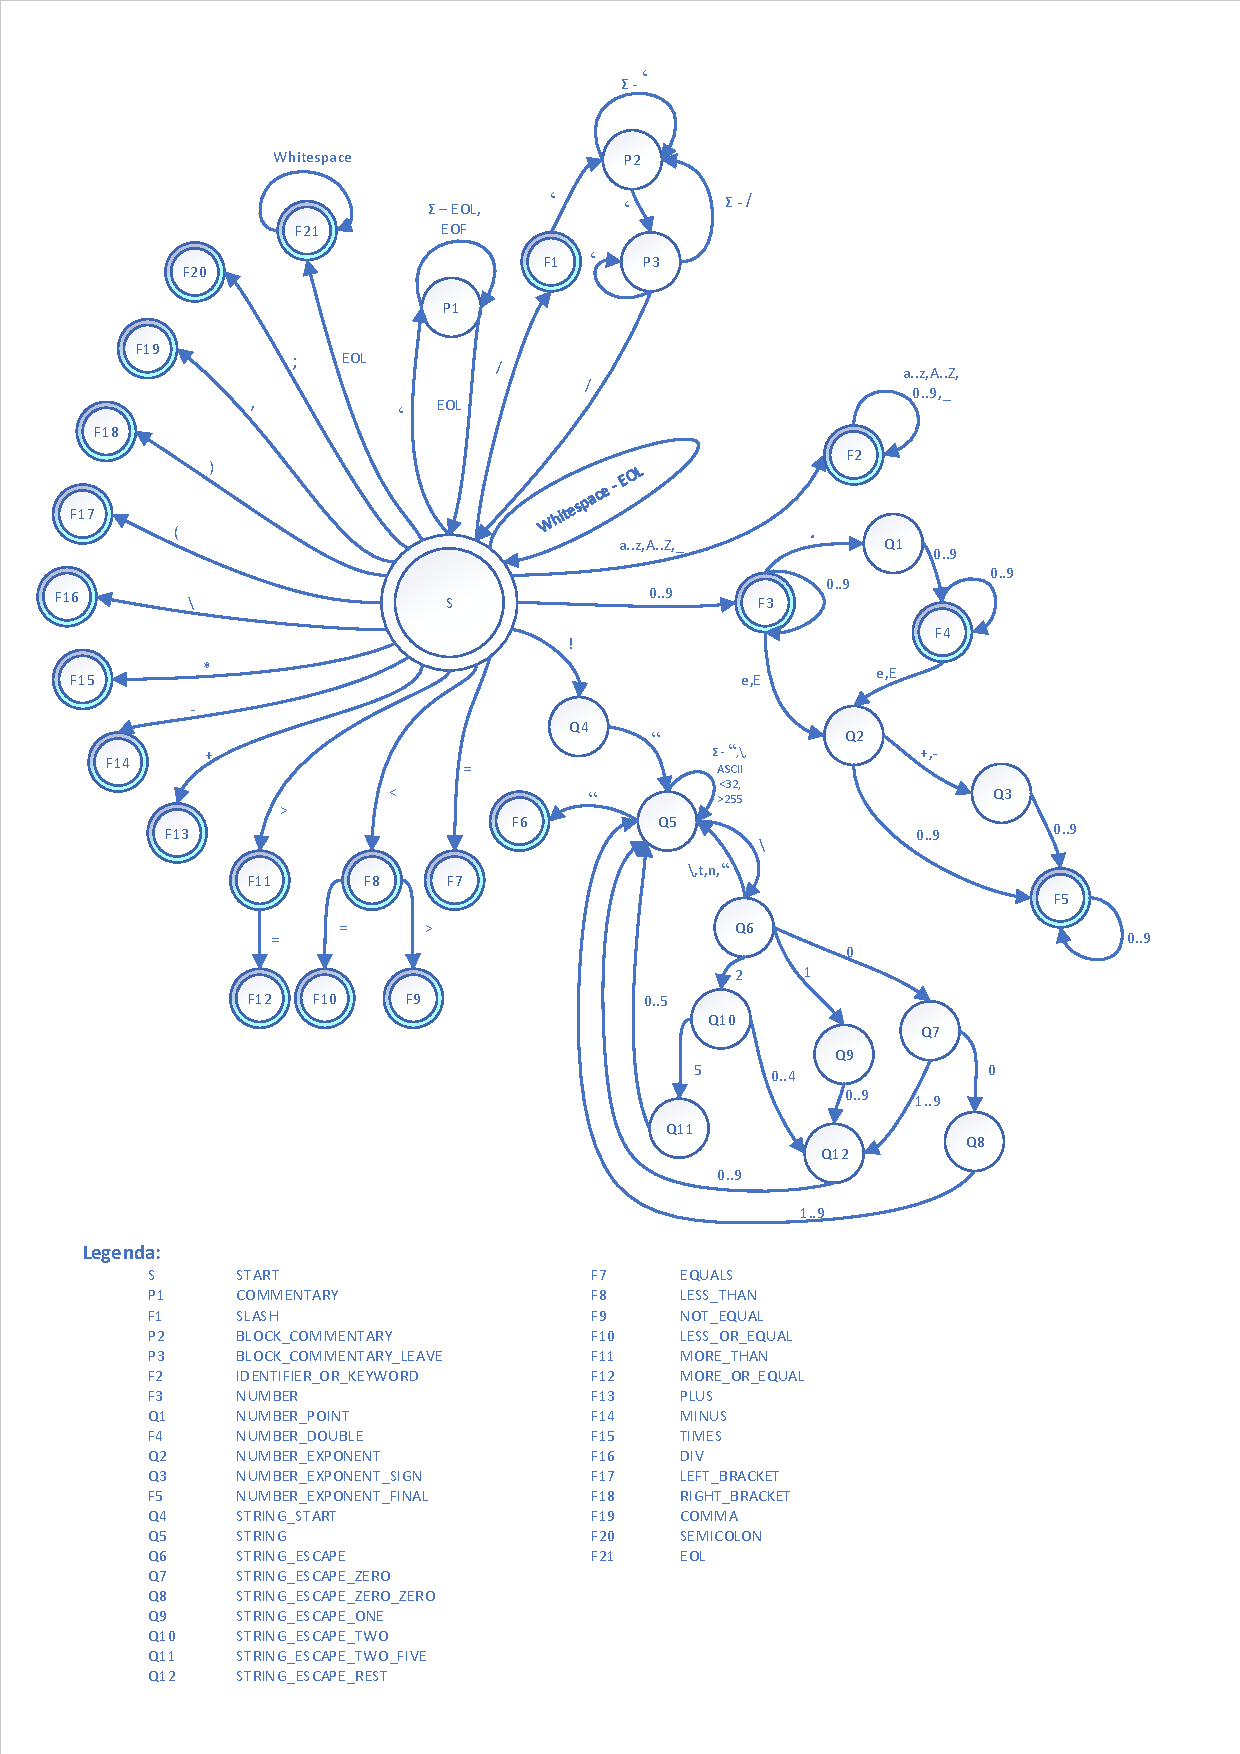
\includegraphics[width=0.95\linewidth]{inc/FA_graph.pdf}
		\caption{Diagram konečného automatu specifikující lexikální analyzátor}
		\label{figure:fa_graph}
	\end{figure}
	\newpage

	\section{LL-gramatika}

	TODO


	\section{LL-tabulka}

	TODO


	\section{Precedenční tabulka}

	TODO

\end{document}
